% !TeX program = xelatex
\documentclass[a4paper,10pt]{article}

% ============================================================================
% កញ្ចប់បណ្ណាល័យ (Packages) – តាមលំនាំស្តង់ដារ អនុវិទ្យាល័យព្រះក្រសាំង (ls_plan.tex)
% បរិបទ៖ ថ្នាក់រៀនគ្មានស្លាយ LCD – បង្រៀនដោយប្រើក្ដារខៀន សៀវភៅគោល និងសន្លឹកកិច្ចការស-ខ្មៅ
% ============================================================================
\usepackage[a4paper, left=0.95cm, right=0.95cm, top=0.85cm, bottom=0.92cm, footskip=0.52cm]{geometry}
\usepackage{amsmath}
\usepackage{unicode-math}
\usepackage{fontspec}
\usepackage{array, longtable, multirow, colortbl}
\usepackage[table]{xcolor}
\usepackage{enumitem}
\usepackage{pifont}
\usepackage{fancyhdr}
\usepackage{tikz}
\usetikzlibrary{calc, arrows.meta, positioning, babel}

\makeatletter
\let\@expl@@@mark@update@singlecol@structures@@\relax
\makeatother

\providecommand{\NGSFindFonts}{%
  \IfFileExists{C:/Windows/Fonts/cambria.ttc}{%
    \def\NGSSysPath{C:/Windows/Fonts/}%
    \def\NGSUserPath{C:/Users/KIT/AppData/Local/Microsoft/Windows/Fonts/}%
  }{%
    \IfFileExists{./fonts/KhmerOSsiemreap.ttf}{\def\NGSSysPath{./fonts/}\def\NGSUserPath{./fonts/}}{%
    \IfFileExists{../fonts/KhmerOSsiemreap.ttf}{\def\NGSSysPath{../fonts/}\def\NGSUserPath{../fonts/}}{%
    \IfFileExists{../../fonts/KhmerOSsiemreap.ttf}{\def\NGSSysPath{../../fonts/}\def\NGSUserPath{../../fonts/}}{%
    \IfFileExists{../../../fonts/KhmerOSsiemreap.ttf}{\def\NGSSysPath{../../../fonts/}\def\NGSUserPath{../../../fonts/}}{%
    \IfFileExists{../../../../fonts/KhmerOSsiemreap.ttf}{\def\NGSSysPath{../../../../fonts/}\def\NGSUserPath{../../../../fonts/}}{%
    \IfFileExists{../../../../../fonts/KhmerOSsiemreap.ttf}{\def\NGSSysPath{../../../../../fonts/}\def\NGSUserPath{../../../../../fonts/}}{%
    \IfFileExists{../../../../../../fonts/KhmerOSsiemreap.ttf}{\def\NGSSysPath{../../../../../../fonts/}\def\NGSUserPath{../../../../../../fonts/}}{%
      \def\NGSSysPath{../../../../../../../fonts/}\def\NGSUserPath{../../../../../../../fonts/}%
    }}}}}}}%
  }%
}
\NGSFindFonts

\setmathfont[Path={\NGSSysPath}, FontIndex=1, Scale=1.02]{cambria.ttc}
\defaultfontfeatures{Ligatures=TeX}

\setmainfont[
  Path={\NGSUserPath},
  Extension=.ttf,
  Script=Khmer,
  BoldFont={KhmerOSsiemreap},
  BoldFeatures={FakeBold=1.8},
  ItalicFont={KhmerOSsiemreap},
  ItalicFeatures={FakeSlant=0.25},
  BoldItalicFont={KhmerOSsiemreap},
  BoldItalicFeatures={FakeBold=1.8, FakeSlant=0.25}
]{KhmerOSsiemreap}

\newfontfamily\muol[Path={\NGSUserPath}, Extension=.ttf, Script=Khmer]{KhmerOSmuollight}
\newfontfamily\TimesEn[Path={\NGSSysPath}, Extension=.ttf, BoldFont={timesbd}, ItalicFont={timesi}, BoldItalicFont={timesbi}]{times}
\newfontfamily\NagaBold[Path={\NGSUserPath}, Extension=.ttf]{AKbalthom Naga Bold}
\newfontfamily\CalibriFont[Path={\NGSSysPath}, Extension=.ttf]{calibri}
\newfontfamily\Tacteing[Path={\NGSUserPath}]{TACTENG.TTF}
\newfontfamily\CourierBullet[Path={\NGSSysPath}, Extension=.ttf]{cour}
\newcommand{\wcirc}{{\CourierBullet\fontsize{9.5pt}{11pt}\selectfont o}}

\XeTeXlinebreaklocale "km"
\XeTeXlinebreakskip = 0pt plus 1pt minus 0.1pt

\definecolor{stepgray}{HTML}{D9D9D9}
\definecolor{headgray}{HTML}{F2F2F2}
\definecolor{boxgray}{HTML}{D9D9D9}
\definecolor{darkred}{HTML}{C00000}
\definecolor{red5e}{HTML}{FF0000}

\pagestyle{fancy}
\fancyhf{}
\renewcommand{\headrulewidth}{0pt}
\fancyfoot[R]{\CalibriFont\fontsize{11pt}{13pt}\selectfont\thepage}

\setlength{\parindent}{0pt}
\setlength{\parskip}{0pt}
\setlength{\tabcolsep}{3.8pt}

\newcolumntype{L}[1]{>{\raggedright\arraybackslash}p{#1}}

\newcommand{\en}[1]{{\TimesEn #1}}
\newcommand{\enbf}[1]{{\TimesEn\textbf{#1}}}
\newcommand{\unit}[1]{\,\text{\en{#1}}}
\newcommand{\fiveE}[1]{{\NagaBold\fontsize{9.5pt}{13pt}\selectfont\textcolor{red5e}{#1}}}
\newcommand{\timenote}[1]{\textcolor{darkred}{\textit{#1}}}
\newcommand{\graybox}[1]{\colorbox{boxgray}{\strut\hspace{2pt}#1\hspace{2pt}}}
\newcommand{\ditem}{\tikz[baseline=-0.5ex]\fill (0,0.42ex) -- (0.42ex,0) -- (0,-0.42ex) -- (-0.42ex,0) -- cycle;\hspace{0.3em}}
\newcommand{\cnum}[1]{{\fontsize{10.5pt}{12pt}\selectfont\ding{\numexpr171+#1\relax}}\hspace{0.2em}}
\newcommand{\cfig}[1]{\par\vspace{4pt}{\centering #1\par}\vspace{4pt}}
\newcommand{\stepheader}[1]{\multicolumn{3}{|c|}{\cellcolor{stepgray}\muol #1} \\* \noalign{\hrule height 0.4pt}}
\newcommand{\khmflourish}{{\Tacteing\fontsize{36pt}{14pt}\selectfont\raisebox{-5pt}{3}}}

% ============================================================================
% ម៉ាក្រូរូបភាពគរុកោសល្យស-ខ្មៅ (Proportional B&W TikZ Diagrams)
% ============================================================================

% ១. E1 Engage: អន្ទាក់គូបនៃទ្វេធា (x+1)^3 vs លំនាំមេគុណត្រីកោណប៉ាស្កាល់ (ទំ.៦៦, ៦៨)
\newcommand{\figEngageALGSix}{%
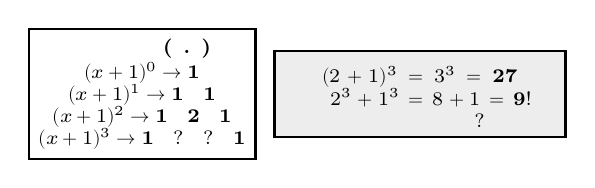
\begin{tikzpicture}[every node/.style={font=\scriptsize, text=black}]
  \node[draw=black, line width=0.9pt, fill=white, inner sep=3.5pt, align=center] (pasc) at (0,0) {
    \textbf{លំនាំមេគុណទ្វេធា (ទំ.៦៨)៖}\\[1pt]
    $(x+1)^0 \to \mathbf{1}$\\
    $(x+1)^1 \to \mathbf{1\quad 1}$\\
    $(x+1)^2 \to \mathbf{1\quad 2\quad 1}$\\
    $(x+1)^3 \to \mathbf{1\quad ?\quad ?\quad 1}$
  };
  \node[draw=black, line width=0.9pt, fill=gray!14, text width=3.45cm, align=center, inner sep=3.5pt, right=6pt of pasc] (trap) {
    \textbf{អន្ទាក់គូបនៃទ្វេធា៖}\\
    $(2+1)^3 = 3^3 = \mathbf{27}$\\
    ខណៈ $2^3 + 1^3 = 8 + 1 = \mathbf{9}$!\\
    តើបាត់តួកណ្ដាលអ្វីខ្លះ?
  };
\end{tikzpicture}}

% ២. E4 Elaborate: ត្រីកោណប៉ាស្កាល់ដល់ជួរទី៥ និងការស៊ីសងតួកណ្ដាលនៃ a^3 ± b^3 (ទំ.៦៧-៦៨)
\newcommand{\figPascalALGSix}{%
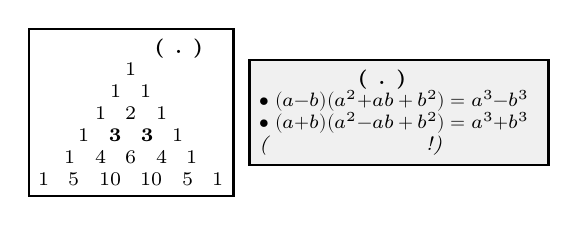
\begin{tikzpicture}[every node/.style={font=\scriptsize, text=black}]
  \node[draw=black, line width=0.9pt, fill=white, inner sep=3.5pt, align=center] (tri) at (0,0) {
    \textbf{ត្រីកោណប៉ាស្កាល់ (ទំ.៦៨)}\\
    $1$\\
    $1 \quad 1$\\
    $1 \quad 2 \quad 1$\\
    $1 \quad \mathbf{3} \quad \mathbf{3} \quad 1$\\
    $1 \quad 4 \quad 6 \quad 4 \quad 1$\\
    $1 \quad 5 \quad 10 \quad 10 \quad 5 \quad 1$
  };
  \node[draw=black, line width=0.8pt, fill=gray!12, text width=3.55cm, align=left, inner sep=3.5pt, right=5pt of tri] {
    \textbf{ច្បាប់សញ្ញាឆ្លាស់ (ទំ.៦៧)៖}\\
    $\bullet$ $(a\mathbf{-}b)(a^2\mathbf{+}ab+b^2) = a^3\mathbf{-}b^3$\\
    $\bullet$ $(a\mathbf{+}b)(a^2\mathbf{-}ab+b^2) = a^3\mathbf{+}b^3$\\
    \textit{(សញ្ញាក្នុងត្រីធាផ្ទុយពីទ្វេធា!)}
  };
\end{tikzpicture}}

\begin{document}
\fontsize{10pt}{15.2pt}\selectfont

% -------------------- ក្បាលកិច្ចតែងការ (Header) --------------------
\begin{center}
  {\muol\fontsize{11pt}{16pt}\selectfont ព្រះរាជាណាចក្រកម្ពុជា}\\[2pt]
  {\muol\fontsize{10pt}{15pt}\selectfont ជាតិ សាសនា ព្រះមហាក្សត្រ}\\[1pt]
  \khmflourish
\end{center}

\vspace{-28pt}
{\muol\fontsize{9.5pt}{12.5pt}\selectfont
មន្ទីរអប់រំ យុវជន និងកីឡា ខេត្តកំពង់ធំ\\
ការិយាល័យអប់រំ យុវជន និងកីឡា ស្រុកកំពង់ស្វាយ\\
អនុវិទ្យាល័យព្រះក្រសាំង}

\vspace{1pt}
\begin{center}
  {\muol\fontsize{10pt}{14pt}\selectfont កិច្ចតែងការបង្រៀន}
\end{center}
\vspace{0pt}

% -------------------- ព័ត៌មានទូទៅ (Metadata) --------------------
{\renewcommand{\arraystretch}{0.95}
\hspace*{4.05cm}%
\begin{tabular}{@{}l l l@{}}
  - \hspace{0.35cm} មុខវិជ្ជា & : & គណិតវិទ្យា ថ្នាក់ទី៨ \\
  - \hspace{0.35cm} ចំណងជើងមេរៀន & : & មេរៀនទី៥ កន្សោមពីជគណិត \\
  - \hspace{0.35cm} ចំណងជើងរង & : & ៣.២ ពន្លាតគូបនៃទ្វេធា ផលបូក-ដកពីរគូប និងត្រីកោណប៉ាស្កាល់ \\
  - \hspace{0.35cm} រយៈពេល & : & ១ ម៉ោងសិក្សា (៥០ នាទី) \\
  - \hspace{0.35cm} បង្រៀនដោយ & : & ហុក ប៊ុនថែន \\
  - \hspace{0.35cm} កាលបរិច្ឆេទ & : & ថ្ងៃព្រហស្បតិ៍ ១កើត ខែមិគសិរ ព.ស.២៥៧០ (១០ ធ្នូ ២០២៦) \\
\end{tabular}
}

\vspace{1pt}

% -------------------- I. វត្ថុបំណង --------------------
\textbf{I.} {\muol វត្ថុបំណង}\\[1pt]
\hspace*{0.55cm}%
\begin{tabular}{@{}l l L{14.2cm}@{}}
  \wcirc \hspace{0.25cm} វិជ្ជាសម្បទា & : & សិស្សប្រាប់បានត្រឹមត្រូវនូវរូបមន្តគូបនៃទ្វេធា $(a\pm b)^3 = a^3 \pm 3a^2b + 3ab^2 \pm b^3$, រូបមន្តបង្កើតផលដក និងផលបូកពីរគូប $(a\mp b)(a^2\pm ab+b^2) = a^3\mp b^3$ ព្រមទាំងរបៀបបង្កើត \textbf{ត្រីកោណប៉ាស្កាល់} (ទំ.៦៦--៦៨) ។ \\
  \wcirc \hspace{0.25cm} បំណិនសម្បទា & : & សិស្សពន្លាតកន្សោមគូបនៃទ្វេធា គណនាផលគុណទ្វេធានឹងត្រីធាឈានទៅ $a^3\pm b^3$ និងប្រើមេគុណត្រីកោណប៉ាស្កាល់ដើម្បីពន្លាត $(x+1)^n$ បានត្រឹមត្រូវ ។ \\
  \wcirc \hspace{0.25cm} ចរិយាសម្បទា & : & សិស្សមានភាពហ្មត់ចត់ក្នុងការសង្កេតសញ្ញាឆ្លាស់គ្នានៃ $(a-b)^3$ និងសញ្ញាផ្ទុយគ្នារវាងទ្វេធា-ត្រីធាក្នុង $a^3\pm b^3$ ព្រមទាំងសហការពិភាក្សាដៃគូយ៉ាងសកម្ម ។ \\
\end{tabular}

\vspace{1pt}

% -------------------- II. សម្ភារៈឧបទេស --------------------
\textbf{II.} {\muol សម្ភារៈឧបទេស}\\[1pt]
\hspace*{0.55cm}$\bullet$ \hspace{0.35cm} សៀវភៅសិក្សាគោលគណិតវិទ្យាថ្នាក់ទី៨ (ទំ.៦៦--៦៨ និងទំ.៧៣) ក្ដារខៀន ដីស បន្ទាត់ និងសន្លឹកកិច្ចការសិស្សស-ខ្មៅ (\en{Worksheet\_ALG56} ចំនួន ២ ទំព័រ \en{A4} ដោយគ្មានស្លាយ \en{LCD}) ។

\vspace{1pt}

% -------------------- III. វិធីសាស្រ្តបង្រៀន --------------------
\textbf{III.} {\muol វិធីសាស្រ្តបង្រៀន}\\[1pt]
\hspace*{0.55cm}$\bullet$ \hspace{0.35cm} គោលវិធីសិស្សមជ្ឈមណ្ឌលតាមគំរូ \en{5Es} រួមបញ្ចូល \textbf{ការរុករកមេគុណត្រីកោណប៉ាស្កាល់ និងការប្រៀបធៀបរចនាសម្ព័ន្ធស៊ីសងតួកណ្ដាល} (\en{Pascal's Triangle Discovery \& Telescoping Sign-Structure Contrast}; \en{Theba et al., 2024; Fitria et al., 2023}) ។

\vspace{2pt}

% -------------------- IV. ដំណើរការបង្រៀន --------------------
\textbf{IV.} {\muol ដំណើរការបង្រៀន}\\[-6pt]

{\renewcommand{\arraystretch}{1.15}
\begin{longtable}{|L{5.50cm}|L{7.90cm}|L{4.80cm}|}
\hline
\multicolumn{1}{|c|}{\cellcolor{headgray}\muol សកម្មភាពគ្រូ} &
\multicolumn{1}{c|}{\cellcolor{headgray}\muol ខ្លឹមសារមេរៀន} &
\multicolumn{1}{c|}{\cellcolor{headgray}\muol សកម្មភាពសិស្ស} \\[2pt]
\hline
\endfirsthead

\hline
\multicolumn{1}{|c|}{\cellcolor{headgray}\muol សកម្មភាពគ្រូ} &
\multicolumn{1}{c|}{\cellcolor{headgray}\muol ខ្លឹមសារមេរៀន} &
\multicolumn{1}{c|}{\cellcolor{headgray}\muol សកម្មភាពសិស្ស} \\[2pt]
\hline
\endhead

\hline
\endfoot

% ==================== ជំហានទី១ (2min) ====================
\stepheader{ជំហានទី១ ៖ រដ្ឋបាលថ្នាក់ (២ នាទី)}
$\bullet$ ពិនិត្យអវត្តមាន សណ្ដាប់ធ្នាប់ អនាម័យ និងសៀវភៅគោល \par\vspace{1pt}
$\bullet$ ចែកសន្លឹកកិច្ចការស-ខ្មៅ \en{Worksheet\_ALG56} ដល់សិស្សគ្រប់គ្នា
&
$\bullet$ វត្តមានសិស្ស ឯកសណ្ឋាន និងសណ្ដាប់ធ្នាប់ថ្នាក់រៀន \par
$\bullet$ សន្លឹកកិច្ចការសិស្ស \en{Worksheet\_ALG56} (ទំព័រ ១--២) លើតុរៀងៗខ្លួន
&
$\circ$ ប្រធានថ្នាក់រាយការណ៍អវត្តមាន \par
$\circ$ សរសេរឈ្មោះលើសន្លឹកកិច្ចការ \\
\hline

% ==================== ជំហានទី២ (9min) ====================
\stepheader{ជំហានទី២ ៖ កែកិច្ចការផ្ទះ រំលឹកមេរៀនចាស់ និងភ្ជាប់បញ្ហាថ្មី (៩ នាទី)}
\ditem \textbf{កែកិច្ចការផ្ទះ ($\le 3\unit{min}$)៖} \par
$\bullet$ ហៅសិស្ស ១ រូបឡើងកែលំហាត់ ៨ក និង ៩ ($54^2-46^2$) ទំ.៧៣ លើក្ដារខៀន
&
\textbf{កំណែកិច្ចការផ្ទះ (សៀវភៅគោល ទំ.៧៣)៖} \par
១) $(1+x)(1-x)(1+x^2) = (1-x^2)(1+x^2) = 1^2 - (x^2)^2 = \mathbf{1 - x^4}$ (ពិត) ។ \par
២) $54^2 - 46^2 = (54-46)(54+46) = 8 \times 100 = \mathbf{800}$ ។
&
$\circ$ ផ្ទៀងផ្ទាត់ការប្រើ $(a-b)(a+b)=a^2-b^2$ ពីរដងជាប់គ្នា \\[3pt]

\ditem \textbf{រំលឹកមេរៀនចាស់ ($3\unit{min}$)៖} \par
$\bullet$ សួររំលឹកពីសមភាព $(a\pm b)^2$ និងការលើកឯកធាជាគូប $(2x)^3,\; (\sqrt{2}a)^3$
&
\textbf{សំណួររំលឹកមូលដ្ឋានគ្រឹះ៖} \par
១) រូបមន្ត៖ $(a+b)^2 = a^2+2ab+b^2$ \;;\; $(a-b)^2 = a^2-2ab+b^2$ ។ \par
២) គូបនៃឯកធា៖ $(2x)^3 = \mathbf{8x^3}$ \;;\; $(3y)^3 = \mathbf{27y^3}$ \;;\; $\left(\frac{1}{5}a\right)^3 = \mathbf{\frac{1}{125}a^3}$ ។
&
$\circ$ ឆ្លើយរំលឹករូបមន្តការេនៃទ្វេធា និងការលើកមេគុណជាគូប \\[3pt]

\fiveE{E1 - Engage} \timenote{(3 នាទី)} \par\vspace{1pt}
$\bullet$ សរសេរលំនាំមេគុណ $(x+1)^0, (x+1)^1, (x+1)^2$ និងអន្ទាក់ $(2+1)^3 \ne 2^3+1^3$ លើក្ដារខៀន រួចឱ្យសិស្សទស្សន៍ទាយមេគុណជួរទី៣
&
\textbf{ស្ថានភាពភ្ជាប់បញ្ហា៖ អាថ៌កំបាំងមេគុណទ្វេធា និងអន្ទាក់គូបនៃផលបូក!} \par
ម្សិលមិញ $(x+1)^2 = 1x^2 + 2x + 1$ មានមេគុណ \textbf{$1,\; 2,\; 1$} ។ បើយើងគិត $(2+1)^3 = 3^3 = \mathbf{27}$ ខណៈ $2^3 + 1^3 = 8 + 1 = \mathbf{9}$ (ខ្វះដល់ទៅ $18$)! \par
\hspace*{0.3em}– \textbf{សំណួរបេសកកម្ម៖} «តើមេគុណនៃ $(x+1)^3$ គឺជា $1, 2, 2, 1$ ឬជា $\mathbf{1, 3, 3, 1}$? ហើយកន្សោមណាទើបគុណទៅសល់ត្រឹម $a^3 - b^3$?»
&
$\circ$ សង្កេតលំនាំបូកមេគុណជួរលើ $1+2=3$ \par
$\circ$ គូសធីកការទស្សន៍ទាយមុនរៀនក្នុងផ្នែកទី១ នៃសន្លឹកកិច្ចការ \\[3pt]

& \cfig{\figEngageALGSix} & \\
\hline

% ==================== ជំហានទី៣ (17min) ====================
\stepheader{ជំហានទី៣ ៖ មេរៀនថ្មី — ពន្លាតគូបនៃទ្វេធា និងត្រីកោណប៉ាស្កាល់ (១៧ នាទី)}
\fiveE{E2 - Explore} \timenote{(11 នាទី)} \par\vspace{1pt}
\ditem \textbf{សកម្មភាពទី១៖ រុករកគូបនៃផលបូក និងគូបនៃផលដក ($5.5\unit{min}$)៖} \par
$\bullet$ ឱ្យសិស្សធ្វើការជាដៃគូលើ \textbf{ផ្នែកទី២ (ក)} នៃ \en{Worksheet\_ALG56} ដើម្បីគុណពន្លាត $(a+b)^2(a+b)$ និង $(a-b)(a-b)^2$ (ទំ.៦៦--៦៧)
&
\textbf{ការរុករកទី១ (ពន្លាត $(a+b)^3$ និង $(a-b)^3$ ទំ.៦៦--៦៧)៖} \par
$\bullet$ $(a+b)^3 = (a^2+2ab+b^2)(a+b) = a^3 + 2a^2b + ab^2 + a^2b + 2ab^2 + b^3 = \mathbf{a^3 + 3a^2b + 3ab^2 + b^3}$ \en{(4)} ។ \par
$\bullet$ $(a-b)^3 = (a-b)(a^2-2ab+b^2) = \mathbf{a^3 - 3a^2b + 3ab^2 - b^3}$ \en{(5)} \textit{(សញ្ញាឆ្លាស់គ្នា៖ $+,\; -,\; +,\; -$!)} ។
&
$\circ$ គុណពន្លាត និងបង្រួម $2a^2b + a^2b = 3a^2b$ \par
$\circ$ កត់សម្គាល់សញ្ញាឆ្លាស់គ្នា $+, -, +, -$ ក្នុង $(a-b)^3$ \\[3pt]

\ditem \textbf{សកម្មភាពទី២៖ រុករកផលគុណបង្កើត $a^3 - b^3$ និង $a^3 + b^3$ ($5.5\unit{min}$)៖} \par
$\bullet$ ឱ្យដៃគូបន្តបំពេញ \textbf{ផ្នែកទី២ (ខ)}៖ គុណ $(a-b)(a^2+ab+b^2)$ និង $(a+b)(a^2-ab+b^2)$ ដោយគូសឈូតតួផ្ទុយគ្នា (ទំ.៦៧)
&
\textbf{ការរុករកទី២ (ការស៊ីសងតួកណ្ដាលឈានទៅ $a^3 \mp b^3$ ទំ.៦៧)៖} \par
$\bullet$ $(a-b)(a^2+ab+b^2) = a^3 + a^2b + ab^2 - a^2b - ab^2 - b^3 = \mathbf{a^3 - b^3}$ \en{(6)} ។ \par
$\bullet$ $(a+b)(a^2-ab+b^2) = a^3 - a^2b + ab^2 + a^2b - ab^2 + b^3 = \mathbf{a^3 + b^3}$ \en{(7)} ។ \par
\textit{(តួកណ្ដាលទាំង ៤ ស៊ីសងគ្នាអស់សូន្យ ព្រោះត្រីធាមានត្រឹម $\mp ab$ មិនមែន $\mp 2ab$!)}
&
$\circ$ គូសឈូតគូតួផ្ទុយគ្នាទាំង ៤ ក្នុងសន្លឹកកិច្ចការ \par
$\circ$ ប្រៀបធៀបសញ្ញាទ្វេធា និងត្រីធារវាងរូបមន្ត \en{(6)} និង \en{(7)} \\[3pt]

\fiveE{E3 - Explain} \timenote{(6 នាទី)} \par\vspace{1pt}
$\bullet$ ហៅតំណាងដៃគូឡើងសង្ខេបសមភាពគូប \en{(4)--(5)} និងសញ្ញាឆ្លាស់គ្នាលើក្ដារខៀន
&
\textbf{សង្ខេបខ្លឹមសារគោល៖ សមភាពគូប \en{(4)--(7)} និងត្រីកោណប៉ាស្កាល់ (ទំ.៦៦--៦៨)} \par
$\bullet$ \cnum{1} \textbf{គូបនៃផលបូក \en{(4)}៖} $(a + b)^3 = a^3 + 3a^2b + 3ab^2 + b^3$ ។ \par
$\bullet$ \cnum{2} \textbf{គូបនៃផលដក \en{(5)}៖} $(a - b)^3 = a^3 - 3a^2b + 3ab^2 - b^3$ (សញ្ញាឆ្លាស់ $+, -, +, -$) ។
&
$\circ$ ឡើងសរសេរសមភាព \en{(4)} និង \en{(5)} លើក្ដារខៀន \\[3pt]

$\bullet$ សង្ខេបរូបមន្តផលដក-ផលបូកពីរគូប \en{(6)--(7)} និងណែនាំ \textbf{ត្រីកោណប៉ាស្កាល់} (ទំ.៦៨)
&
$\bullet$ \cnum{3} \textbf{ផលដកពីរគូប \en{(6)}៖} $(a - b)(a^2 + ab + b^2) = a^3 - b^3$ (ទ្វេធាដក $\to$ ផលដកគូប) ។ \par
$\bullet$ \cnum{4} \textbf{ផលបូកពីរគូប \en{(7)}៖} $(a + b)(a^2 - ab + b^2) = a^3 + b^3$ (ទ្វេធាបូក $\to$ ផលបូកគូប) ។ \par
$\bullet$ \cnum{5} \textbf{ត្រីកោណប៉ាស្កាល់ (ទំ.៦៨)៖} មេគុណជួរបន្ទាប់បានពីបូកមេគុណពីរជាប់គ្នានៅជួរលើ ។
&
$\circ$ កត់ត្រារូបមន្ត \cnum{1}--\cnum{5} ចូលក្នុងប្រអប់ផ្នែកទី៣ \par
$\circ$ បំពេញមេគុណត្រីកោណប៉ាស្កាល់ដល់ជួរ $(x+1)^5$ \\
\hline

% ==================== ជំហានទី៤ (20min) ====================
\stepheader{ជំហានទី៤ ៖ ពង្រីកចំណេះដឹង និងវាយតម្លៃលទ្ធផលសិក្សា (២០ នាទី)}
\fiveE{E4 - Elaborate} \timenote{(10 នាទី)} \par\vspace{1pt}
\ditem \textbf{លំហាត់គំរូពន្លាតគូប និងផលបូក-ដកពីរគូប (ទំ.៦៦--៦៧, $5\unit{min}$)៖} \par
$\bullet$ ដឹកនាំសិស្សដោះស្រាយលំហាត់គំរូទាំង ៤ និងករណីមានប្រភាគ/រ៉ាឌីកាល់ក្នុង \textbf{ផ្នែកទី៤ (១)} នៃសន្លឹកកិច្ចការ
&
\textbf{លំហាត់គំរូតាមសៀវភៅគោល (ទំ.៦៦--៦៧)៖} \par
$\bullet$ គំរូ \en{(4)--(5)}៖ $(x+1)^3 = \mathbf{x^3 + 3x^2 + 3x + 1}$ \;;\; $(x-1)^3 = \mathbf{x^3 - 3x^2 + 3x - 1}$ ។ \par
$\bullet$ គំរូ \en{(6)--(7)}៖ $(x-1)(x^2+x+1) = \mathbf{x^3 - 1}$ \;;\; $(x+1)(x^2-x+1) = \mathbf{x^3 + 1}$ ។ \par
$\bullet$ អនុវត្តមេគុណប្រភាគ៖ $\left(\frac{1}{5}a + b\right)^3 = \mathbf{\frac{1}{125}a^3 + \frac{3}{25}a^2b + \frac{3}{5}ab^2 + b^3}$ ។ \par
$\bullet$ អនុវត្តរ៉ាឌីកាល់ (ទំ.៦៧)៖ $(\sqrt{2}a - 3b)(2a^2 + 3\sqrt{2}ab + 9b^2) = (\sqrt{2}a)^3 - (3b)^3 = \mathbf{2\sqrt{2}a^3 - 27b^3}$ ។
&
$\circ$ ផ្ទៀងផ្ទាត់ថាត្រីធា $2a^2 + 3\sqrt{2}ab + 9b^2$ ត្រូវនឹងទម្រង់ $A^2 + AB + B^2$ មុនប្រើរូបមន្ត \en{(6)} \\[3pt]

\ditem \textbf{អនុវត្តត្រីកោណប៉ាស្កាល់ដល់ដឺក្រេទី ៥ (ទំ.៦៨, $5\unit{min}$)៖} \par
$\bullet$ ដឹកនាំសិស្សបង្កើតជួរទី៤ និងទី៥ នៃត្រីកោណប៉ាស្កាល់ ដើម្បីពន្លាត $(x+1)^4$ និង $(x+1)^5$ (ទំ.៦៨)
&
\textbf{ការពន្លាតតាមត្រីកោណប៉ាស្កាល់ (សៀវភៅគោល ទំ.៦៨)៖} \par
$\bullet$ ជួរទី៤ ($1, 4, 6, 4, 1$)៖ $(x+1)^4 = \mathbf{x^4 + 4x^3 + 6x^2 + 4x + 1}$ ។ \par
$\bullet$ ជួរទី៥ ($1, 5, 10, 10, 5, 1$)៖ $(x+1)^5 = \mathbf{x^5 + 5x^4 + 10x^3 + 10x^2 + 5x + 1}$ ។ \par
$\bullet$ គិតមាត់តាមរូបមន្ត \en{(4)}៖ $11^3 = (10+1)^3 = 1000 + 300 + 30 + 1 = \mathbf{1331}$ ។ \par
$\bullet$ \textbf{ឆ្លុះបញ្ចាំង៖} ក្នុងពន្លាត $(a+b)^n$ និទស្សន្តនៃ $a$ ថយចុះពី $n\to 0$ ឯនិទស្សន្តនៃ $b$ កើនឡើងពី $0\to n$ ។
&
$\circ$ បូកមេគុណជួរទី៤ បាន $1, 5, 10, 10, 5, 1$ សម្រាប់ $(x+1)^5$ \\[3pt]

& \cfig{\figPascalALGSix} & \\[3pt]

\fiveE{E5 - Evaluate} \timenote{(10 នាទី)} \par\vspace{1pt}
\ditem \textbf{អនុវត្ត «ប្រតិបត្តិ» ទំ.៦៦ និងទំ.៦៧ ($6.5\unit{min}$)៖} \par
$\bullet$ ឱ្យសិស្សធ្វើលំហាត់ \textbf{ប្រតិបត្តិ} គូបនៃទ្វេធា (ទំ.៦៦--៦៧) ដោយខ្លួនឯងក្នុងផ្នែកទី៥ (១) នៃសន្លឹកកិច្ចការ
&
\textbf{ចម្លើយលំហាត់ «ប្រតិបត្តិ» (សៀវភៅគោល ទំ.៦៦--៦៧)៖} \par
១) \textbf{គូបនៃទ្វេធា \en{(4)--(5)}៖} ក) $(x+2y)^3 = \mathbf{x^3 + 6x^2y + 12xy^2 + 8y^3}$ \;;\; ខ) $(3x+4y)^3 = \mathbf{27x^3 + 108x^2y + 144xy^2 + 64y^3}$ \;;\; គ) $(3x-2y)^3 = \mathbf{27x^3 - 54x^2y + 36xy^2 - 8y^3}$ \;;\; ឃ) $(2x-y)^3 = \mathbf{8x^3 - 12x^2y + 6xy^2 - y^3}$ ។
&
$\circ$ ពន្លាតដោយប្រយ័ត្ន $(2y)^3 = 8y^3$ និងសញ្ញាឆ្លាស់ $+, -, +, -$ \\[3pt]

$\bullet$ ឱ្យសិស្សបន្តធ្វើ \textbf{ប្រតិបត្តិ} រូបមន្ត \en{(6)--(7)} (ទំ.៦៧) រួចប្ដូរសន្លឹកកិច្ចការផ្ទៀងជាដៃគូ
&
២) \textbf{ផលដក និងផលបូកពីរគូប \en{(6)--(7)} (ទំ.៦៧)៖} \par
\hspace*{0.3em}– $(x-3)(x^2+3x+9) = \mathbf{x^3 - 27}$ \quad;\quad $(2x-1)(4x^2+2x+1) = \mathbf{8x^3 - 1}$ \par
\hspace*{0.3em}– $(x+3)(x^2-3x+9) = \mathbf{x^3 + 27}$ \quad;\quad $(2x+1)(4x^2-2x+1) = \mathbf{8x^3 + 1}$ ។
&
$\circ$ ប្ដូរសន្លឹកកិច្ចការផ្ទៀងផ្ទាត់ $(2x)^3 = 8x^3$ និងសញ្ញា $\mp 1$ (\en{Pause-Review}) \\[3pt]

\ditem \textbf{បិទបេសកកម្ម E1 និងតេស្តរហ័ស \en{Exit Check} ($3.5\unit{min}$)៖} \par
$\bullet$ សួរបិទបេសកកម្ម E1 និងឱ្យសិស្សគូសរង្វង់ជម្រើស \en{A--D}
&
$\bullet$ \textbf{បិទបេសកកម្ម E1៖} មេគុណនៃ $(x+1)^3$ គឺ $\mathbf{1, 3, 3, 1}$ ហើយ $(2+1)^3 = 8+12+6+1 = 27$ ។ \par
$\bullet$ \textbf{Exit Check៖} តើផលគុណ $(2x + 3)(4x^2 - 6x + 9)$ ស្មើនឹងកន្សោមមួយណា? \par
\en{A.} $8x^3 - 27$ \quad \en{B.} $2x^3 + 27$ \quad \graybox{\enbf{C.} $8x^3 + 27$ \ding{51}} \quad \en{D.} $8x^3 + 12x^2 + 27$
&
$\circ$ សម្គាល់ទម្រង់ $(A+B)(A^2-AB+B^2)=A^3+B^3$ រួចគូសរង្វង់ជម្រើស \textbf{C} \\
\hline

% ==================== ជំហានទី៥ (<=2min) ====================
\stepheader{ជំហានទី៥ ៖ កិច្ចការផ្ទះ និងបណ្ដាំផ្ញើ ($\le$ ២ នាទី)}
$\bullet$ កត់ត្រាកិច្ចការផ្ទះលើក្ដារខៀន (មានបោះពុម្ពស្រាប់នៅផ្នែកទី៦ នៃសន្លឹកកិច្ចការទំព័រទី២) \par
$\bullet$ រំលឹកឱ្យដាក់វង់ក្រចកពេលដកកន្សោម $-(x+2)^3$ ក្នុងលំហាត់ ១០ង
&
\textbf{កិច្ចការផ្ទះ (សៀវភៅសិក្សាគោល ទំ.៦៦--៦៧ និងទំ.៧៣)៖} \par
១. \textbf{ប្រតិបត្តិ ឃ (ទំ.៦៦ និងទំ.៦៧)៖} ពន្លាត $\left(\frac{1}{5}a + b\right)^3$, $\left(\frac{1}{5}t - k\right)^3$ និង $(\sqrt{2}a + 3b)(2a^2 - 3\sqrt{2}ab + 9b^2)$ ។ \par
២. \textbf{លំហាត់ទី១០ ង (ទំ.៧៣)៖} ពន្លាត និងបង្រួមតាមលំដាប់ដឺក្រេ៖ $(x - 1)^3 - (x + 2)^3$ ។ \par
៣. \textbf{ត្រីកោណប៉ាស្កាល់៖} រកជួរទី៦ នៃត្រីកោណប៉ាស្កាល់ រួចសរសេរពន្លាតនៃ $(x + 1)^6$ ។
&
$\circ$ កត់ត្រាកិច្ចការផ្ទះ និងទុកដាក់សន្លឹកកិច្ចការក្នុងសឺមីគណិតវិទ្យា \\[3pt]

$\bullet$ ណែនាំឱ្យអានចំណុច ៤.១ និង ៤.២ ជាមុនសម្រាប់ម៉ោងក្រោយ
&
$\bullet$ \textbf{អានជាមុន៖} ចំណុច \textbf{៤.១ និង ៤.២ ការដាក់ជាផលគុណកត្តាដោយកត្តារួម និងតាមសមភាពសំខាន់ៗ} (សៀវភៅគោល ទំព័រ ៦៨--៧០) ។
&
$\circ$ ទទួលបណ្ដាំផ្ញើ និងជម្រាបលាគ្រូ \\

\end{longtable}
}

\vspace{6pt}

% -------------------- ហត្ថលេខា (Signature Block) --------------------
\begin{flushright}
\begin{minipage}{9.6cm}
\centering
ថ្ងៃព្រហស្បតិ៍ ១កើត ខែមិគសិរ ឆ្នាំមមី អដ្ឋស័ក ពុទ្ធសករាជ ២៥៧០\\[2pt]
ព្រះក្រសាំង, ថ្ងៃទី១០ ខែធ្នូ ឆ្នាំ២០២៦\\[4pt]
{\muol គ្រូបង្រៀន}\\[32pt]
\hfill{\muol ហុក ប៊ុនថែន}\hspace*{1.4cm}
\end{minipage}
\end{flushright}

\end{document}
